\documentclass[letterpaper]{article}

\usepackage{flairs}

\usepackage{times}
\usepackage{helvet}
\usepackage{courier}
\frenchspacing
\setlength{\pdfpagewidth}{8.5in}
\setlength{\pdfpageheight}{11in}

\usepackage{graphicx}
\graphicspath{{./images/}}
\usepackage{float}
\usepackage{verbatim}
\usepackage{amssymb}
\usepackage{tikz}
\usetikzlibrary{arrows.meta,positioning}

\pdfinfo{
/Title (Non-Stationary Spectral Decomposition Network for Econometric Time Series Forecasting)
/Author (Nikhil Sunder)
/Keywords(Machine Learning, Neural Networks, Nonstationary Time Series Forecasting, Spectral Decomposition, Neural State-Space Models, Instantaneous Frequency Analysis, Hilbert–Huang Transform, Sinusoidal Neural Networks, Economic Time Series, Latent Dynamical Systems)
}
\setcounter{secnumdepth}{0}

\title{Non-Stationary Spectral Decomposition Network for Econometric Time Series Forecasting}
\author{Nikhil Sunder\\
Miami Herbert Business School,\\
University of Miami, Coral Gables, Florida, USA\\
Email: nss106@miami.edu}

\begin{document}
\maketitle

\begin{abstract}
\begin{quote}
Economic and financial time series frequently exhibit persistent trends along with cyclical dynamics whose amplitude, frequency and phase evolve over time due to structural change, policy shocks, and regime transitions. Traditional forecasting models often impose fixed spectral structure or linear dynamics, limiting their ability to represent such nonstationary behavior. This paper introduces the Non-Stationary Spectral Decomposition Network (NS-SDN), a neural state-space architecture designed to model time series as a sum of time-varying sinusoidal components driven by a latent dynamical state. The model learns trend, amplitude, instantaneous frequency, and phase parameters from latent state transitions and synthesizes observations through a spectral emission equation. This formulation combines ideas from implicit neural representations, instantaneous-frequency analysis, and state-space econometric models. Preliminary experiments on financial time series demonstrate stable training and coherent spectral structure, suggesting that state-driven spectral representations may provide a promising framework for forecasting nonstationary economic dynamics.
\end{quote}
\end{abstract}

\section{Introduction}

Economic and financial time series often exhibit persistent trends alongside cyclical dynamics whose amplitude, duration, and frequency evolve over time. Structural change, policy interventions, and market regime shifts can produce behavior that is difficult to capture with models that assume stationary dynamics or a fixed spectral structure.

Structural time-series and state-space approaches address part of this problem by decomposing observations into latent components such as trend and cycle \cite{harvey1989structural,durbin2012statespace}. However, these models often impose fixed or weakly time-varying cycle frequencies. Time-varying parameter models and regime-switching frameworks partially relax these assumptions, but typically remain linear and rely on strong parametric structure \cite{lubik2015tvpvar,hamilton1989regime}.

Recent work on implicit neural representations shows that sinusoidal nonlinearities can represent complex oscillatory patterns efficiently \cite{sitzmann2020siren}, while the Hilbert--Huang Transform describes nonstationary signals through time-varying amplitude and instantaneous frequency \cite{huang1998hht}. Motivated by these ideas, we introduce the \textit{Non-Stationary Spectral Decomposition Network} (NS-SDN), a neural state-space architecture that models a time series as a sum of sinusoidal components with amplitude, frequency, and phase driven by a latent dynamical state.

\section{Non-Stationary Spectral Decomposition Network}

\subsection{Spectral Decomposition Representation}

Rather than assuming stationary periodic structure, the proposed model represents a time series as a sum of sinusoidal components whose amplitude, frequency, and phase vary over time:

\begin{equation}
\hat{y}_t = B_t + \sum_{k=1}^{K} A_{t,k}\sin(\theta_{t,k} + \phi_{t,k})
\alt{Observation modeled as a sum of a low-frequency trend component and multiple sinusoidal components whose amplitudes, phases, and frequencies vary over time.}
\end{equation}

Here, $B_t$ is a low-frequency trend component, $A_{t,k}$ is the amplitude of component $k$, $\theta_{t,k}$ is cumulative phase, and $\phi_{t,k}$ is a phase offset. This representation is related to instantaneous-frequency decompositions such as the Hilbert--Huang Transform, where signals are interpreted as sums of oscillatory modes with evolving envelopes and frequencies \cite{huang1998hht}. 

\subsection{State-Space Dynamics}

The spectral parameters are generated through a latent dynamical state. Let $h_t \in \mathbb{R}^d$ denote a latent state evolving according to

\begin{equation}
h_t = F_{\psi}(h_{t-1}, x_t, \Delta t)
\alt{Latent state updated through a learned nonlinear transition function of the previous state, current inputs, and time increment.}
\end{equation}

where $F_{\psi}$ is a learned transition function, $x_t$ represents available information at time $t$, and $\Delta t$ denotes the time increment between observations. This formulation follows the structure of nonlinear state-space models commonly used in econometric analysis \cite{durbin2012statespace}.

Given the latent state, the model emits spectral parameters through neural projection heads,

\begin{equation}
B_t, A_t, \omega_t, \phi_t = g_{\psi}(h_t)
\alt{Trend, amplitude, instantaneous frequency, and phase parameters generated as functions of the latent state through a neural projection mapping.}
\end{equation}

where $\omega_{t,k}$ denotes instantaneous angular frequency for component $k$. Phase evolves through discrete-time integration,

\begin{equation}
\theta_{t,k} = \theta_{t-1,k} + \omega_{t,k}\Delta t
\alt{Cumulative phase updated by integrating instantaneous angular frequency over the time increment in discrete time.}
\end{equation}

allowing oscillatory components to adapt dynamically as the latent state evolves. The resulting architecture combines ideas from neural implicit representations with interpretable spectral synthesis, producing a forecasting model capable of representing nonstationary cyclical behavior \cite{sitzmann2020siren}.

\begin{figure}[t]
\centering
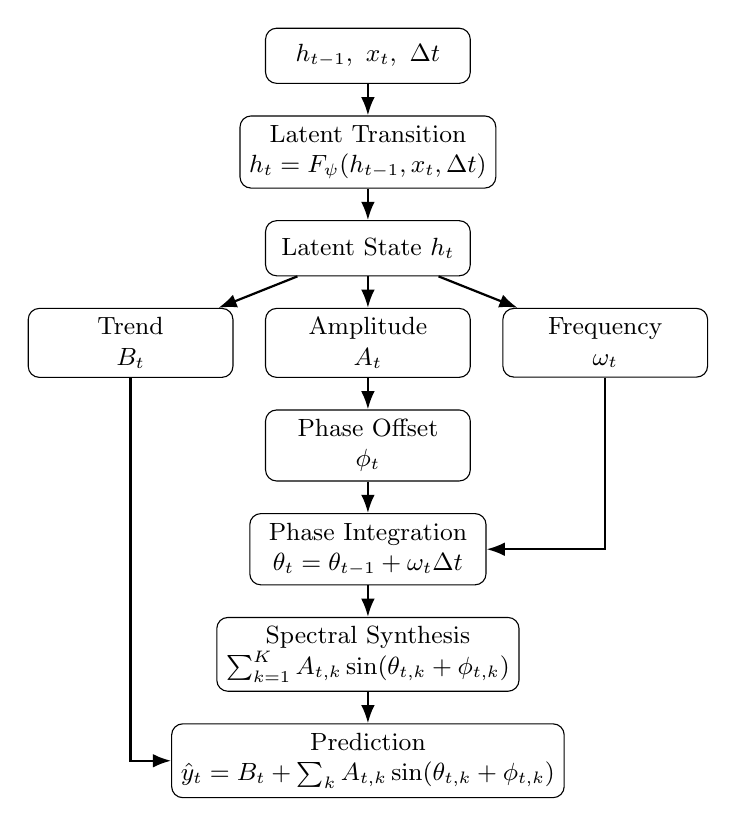
\begin{tikzpicture}[
    node distance=0.4cm,
    >=Latex,
    every node/.style={font=\small},
    box/.style={
        draw,
        rounded corners,
        align=center,
        minimum width=3cm,
        minimum height=0.8cm
    },
    smallbox/.style={
        draw,
        rounded corners,
        align=center,
        minimum width=2.6cm,
        minimum height=0.7cm
    },
    line/.style={->, thick}
]

% Inputs
\node[smallbox] (input) {$h_{t-1},\ x_t,\ \Delta t$};

% Transition
\node[box, below=of input] (transition)
{Latent Transition\\
$h_t = F_{\psi}(h_{t-1},x_t,\Delta t)$};

% Latent state
\node[smallbox, below=of transition] (state)
{Latent State $h_t$};

% Emission heads
\node[smallbox, below left=0.4cm and 0.4cm of state] (B)
{Trend\\$B_t$};

\node[smallbox, below=0.4cm of state] (A)
{Amplitude\\$A_t$};

\node[smallbox, below right=0.4cm and 0.4cm of state] (omega)
{Frequency\\$\omega_t$};

\node[smallbox, below=of A] (phi)
{Phase Offset\\$\phi_t$};

% Phase integration
\node[box, below=0.4cm of phi] (theta)
{Phase Integration\\
$\theta_t=\theta_{t-1}+\omega_t\Delta t$};

% Spectral synthesis
\node[box, below=of theta] (synth)
{Spectral Synthesis\\
$\sum_{k=1}^{K} A_{t,k}\sin(\theta_{t,k}+\phi_{t,k})$};

% Output
\node[box, below=of synth] (output)
{Prediction\\
$\hat{y}_t = B_t + \sum_{k} A_{t,k}\sin(\theta_{t,k}+\phi_{t,k})$};

% Arrows
\draw[line] (input) -- (transition);
\draw[line] (transition) -- (state);

\draw[line] (state) -- (B);
\draw[line] (state) -- (A);
\draw[line] (state) -- (omega);

\draw[line] (A) -- (phi);
\draw[line] (omega) |- (theta);
\draw[line] (phi) -- (theta);

\draw[line] (B) |- (output);
\draw[line] (theta) -- (synth);
\draw[line] (synth) -- (output);

\end{tikzpicture}

\alt{Flow diagram of the NS-SDN architecture where inputs $h_{t-1}$, $x_t$, and $\Delta{t}$ are passed through a latent transition function to produce $h_t$, which is then projected into trend, amplitude, frequency, and phase parameters; frequency and phase are integrated to form cumulative phase, sinusoidal components are synthesized using amplitudes and phases, and combined with the trend to produce the final prediction.}

\caption{Vertical architecture of the Non-Stationary Spectral Decomposition Network (NS-SDN).}

\label{fig:nssdn_architecture}
\end{figure}

\section{Training and Forecasting Setup}

The proposed architecture is evaluated in a univariate forecasting setting. Let $\{y_1, y_2, \dots, y_T\}$ denote an observed time series. The model is trained using sequential one-step-ahead prediction, where the latent state is updated at each time step and the network predicts the next observation.

Given observations up to time $t$, the model generates a forecast

\begin{equation}
\hat{y}_{t+1} = f(y_t, h_t)
\alt{Next-step prediction produced as a function of the current observation and latent state.}
\end{equation}

where $h_t$ denotes the latent state after observing $y_t$. Multi-step forecasts are produced recursively by feeding predicted values back into the model. This recursive forecasting strategy is commonly used in neural time-series models and allows evaluation across multiple horizons \cite{flunkert2020deepar}.

Model parameters are estimated by minimizing mean squared prediction error over the training sequence. Spectral parameters such as amplitude and frequency are learned jointly with the latent transition dynamics through gradient-based optimization.

\section{Discussion and Future Work}

While the preliminary results demonstrate the feasibility of the proposed architecture, a comprehensive evaluation requires systematic comparison with established forecasting models. Future work will benchmark the NS-SDN architecture against classical econometric methods such as ARIMA and vector autoregressions, as well as neural forecasting models including recurrent networks and feedforward architectures.

Forecast comparisons will be conducted using rolling-origin evaluation procedures commonly employed in forecasting studies \cite{west1996predictive}. Statistical significance of forecast improvements will be assessed using tests for equal predictive accuracy such as the Diebold-Mariano test \cite{diebold1995accuracy}.

Beyond predictive performance, the interpretability of the learned spectral components provides an additional avenue for analysis. Examining the evolution of amplitude and frequency parameters may offer insight into changes in economic cycle dynamics or regime transitions.

These extensions will form the basis of a larger empirical study evaluating the effectiveness of state-driven spectral decomposition models for econometric forecasting.

\section{Conclusion}

This paper introduced the Non-Stationary Spectral Decomposition Network (NS-SDN), a neural state-space architecture designed to model time series as a sum of latent sinusoidal components with time-varying amplitude, frequency, and phase. By allowing spectral parameters to evolve through a latent dynamical state, the model provides a flexible representation of nonstationary cyclical behavior while maintaining an interpretable decomposition structure. Preliminary validation demonstrates that the architecture can learn stable spectral components and produce coherent forecasts on financial time series. These results suggest that state-driven spectral synthesis offers a promising approach for modeling evolving cyclical dynamics. Future work will conduct systematic forecasting comparisons against classical econometric and neural models using rolling-origin evaluation and formal forecast accuracy tests.

\bibliography{references}
\bibliographystyle{flairs}
\end{document}